%!TeX root=../tese.tex
%("dica" para o editor de texto: este arquivo é parte de um documento maior)
% para saber mais: https://tex.stackexchange.com/q/78101/183146

%% ------------------------------------------------------------------------- %%
\chapter{Resultados}
\label{cap:resultados}
\section{Progressão}

Com a finalização do trabalho e testes se tornando possíveis, foi se tornando visível a progressão da dificuldade de acordo com a performance do jogador, em tempo real de jogo. Quanto mais tempo o jogador consegue passar sem tocar em nenhum projétil inimigo, mais poderosos ficam os geradores inimigos, e se o jogador estiver sendo severamente punido pela dificuldade, os geradores são ajustados de acordo.

Além do desenvolvimento feito dentro do escopo do jogo, foi implementado também um código em \textit{Python} para visualização da progressão na forma de gráficos, onde é simulado o cálculo de dificuldade feito nos geradores e nas fases.

\begin{figure}
    \centering

    \begin{subfigure}{.7\textwidth}
        \centering
        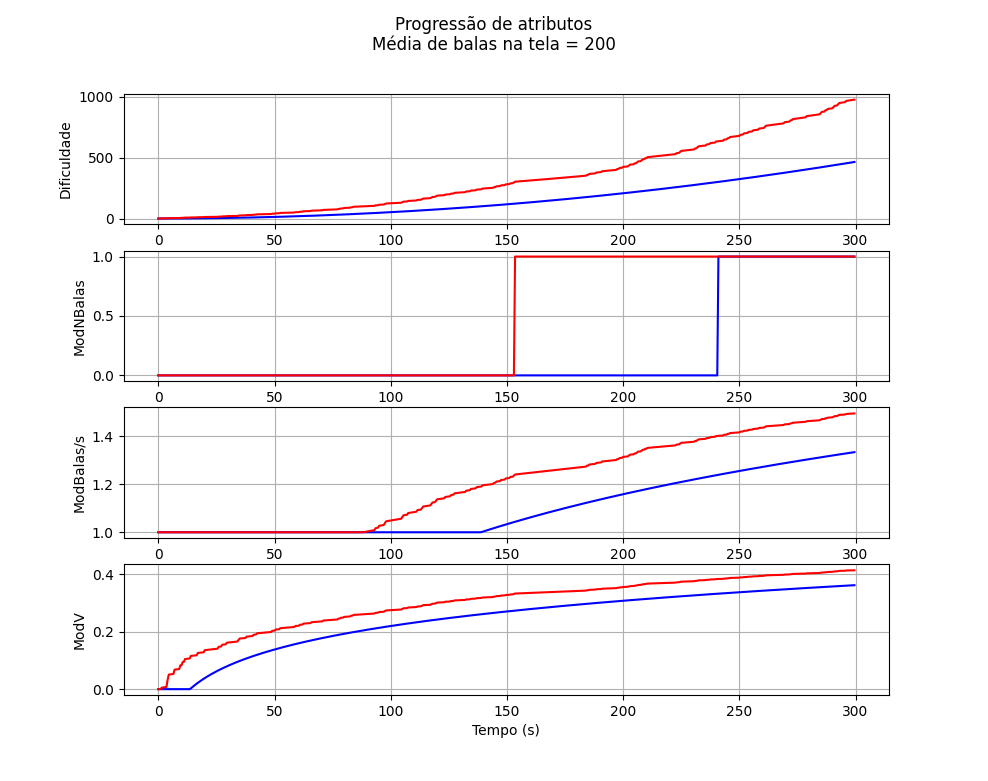
\includegraphics[width=1\textwidth]{graficos}
    \end{subfigure}

    \caption{Gráficos gerados pelo código \textit{graph generator}, o qual pode ser encontrado no repositório do jogo.}
\end{figure}

As simulações apresentadas pelos gráficos envolvem dois casos: progressão da dificuldade considerando uma chance de 15\% a cada meio segundo do personagem realizar um \textit{graze} em uma bala inimiga, em vermelho; e a progressão da dificuldade sem considerar \textit{graze} algum. Ambas simulações consideram um número constante de 200 balas na tela, ao longo de 5 minutos.

O primeiro gráfico mostra a progressão do coeficiente principal de dificuldade, $overall\_difficulty$, este tendo um crescimento quadrático ao longo do tempo, e a progressão dos modificadores calculados dentro dos geradores inimigos.

\section{Considerações}

Com a implementação do sistema funcional, realização de testes e considerações dos estudos feitos, é possível concluir que o uso do balanceamento dinâmico, mesmo que apenas em um protótipo de jogo, é capaz de permitir o acompanhamento da habilidade do jogador em tempo real, esta se encontrando dentro ou não do esperado pelo gênero ou sub-gênero de jogos escolhido no processo de desenvolvimento. Além disso, essa abrangência elevada de atendimento das habilidades pode também vir a poupar o desenvolvedor da pré-programação de dificuldades determinadas, como discutido em \ref{cenario atual}, para atender tais necessidades.

Ainda no ponto de vista do desenvolvedor, a abordagem do sistema estudado é interessante pois proporciona ao desenvolvedor uma tarefa importante: entender os desafios propostos pelo jogo e quais deles merecem atenção e refinamento. Este entendimento se faz importante por englobar uma parte crucial no aproveitamento do jogo, mas também de ser essencial para o desenvolvimento de um sistema de balanceamento dinâmico eficaz. No caso do \textit{Galaxy Rush}, os principais desafios do jogador, considerados pelo cálculo da dificuldade, eram de \textit{desviar de balas inimigas} e \textit{passar o mais perto possível delas}. Esses desafios certamente serão outros em outros gêneros de jogos, evidenciando a importância de seu esclarecimento para o desenvolvedor.

Por outro lado, na perspectiva do jogador, o uso do sistema se torna vantajoso pois evita ao máximo permitir que o jogador esteja em um estado de frustração quanto à dificuldade do jogo. Isso é, a dificuldade atual do jogo nunca estará além das capacidades e habilidades do jogador, cenário que causaria frustração por não permitir que o jogador passe de certos pontos da progressão do jogo, mas também não permite que a dificuldade chegue em um ponto muito abaixo das espectativas, tornando o jogo desinteressante inteiramente.